% Options for packages loaded elsewhere
\PassOptionsToPackage{unicode}{hyperref}
\PassOptionsToPackage{hyphens}{url}
%
\documentclass[
  man,mask,floatsintext]{apa6}
\usepackage{amsmath,amssymb}
\usepackage{iftex}
\ifPDFTeX
  \usepackage[T1]{fontenc}
  \usepackage[utf8]{inputenc}
  \usepackage{textcomp} % provide euro and other symbols
\else % if luatex or xetex
  \usepackage{unicode-math} % this also loads fontspec
  \defaultfontfeatures{Scale=MatchLowercase}
  \defaultfontfeatures[\rmfamily]{Ligatures=TeX,Scale=1}
\fi
\usepackage{lmodern}
\ifPDFTeX\else
  % xetex/luatex font selection
\fi
% Use upquote if available, for straight quotes in verbatim environments
\IfFileExists{upquote.sty}{\usepackage{upquote}}{}
\IfFileExists{microtype.sty}{% use microtype if available
  \usepackage[]{microtype}
  \UseMicrotypeSet[protrusion]{basicmath} % disable protrusion for tt fonts
}{}
\makeatletter
\@ifundefined{KOMAClassName}{% if non-KOMA class
  \IfFileExists{parskip.sty}{%
    \usepackage{parskip}
  }{% else
    \setlength{\parindent}{0pt}
    \setlength{\parskip}{6pt plus 2pt minus 1pt}}
}{% if KOMA class
  \KOMAoptions{parskip=half}}
\makeatother
\usepackage{xcolor}
\usepackage{longtable,booktabs,array}
\usepackage{calc} % for calculating minipage widths
% Correct order of tables after \paragraph or \subparagraph
\usepackage{etoolbox}
\makeatletter
\patchcmd\longtable{\par}{\if@noskipsec\mbox{}\fi\par}{}{}
\makeatother
% Allow footnotes in longtable head/foot
\IfFileExists{footnotehyper.sty}{\usepackage{footnotehyper}}{\usepackage{footnote}}
\makesavenoteenv{longtable}
\usepackage{graphicx}
\makeatletter
\def\maxwidth{\ifdim\Gin@nat@width>\linewidth\linewidth\else\Gin@nat@width\fi}
\def\maxheight{\ifdim\Gin@nat@height>\textheight\textheight\else\Gin@nat@height\fi}
\makeatother
% Scale images if necessary, so that they will not overflow the page
% margins by default, and it is still possible to overwrite the defaults
% using explicit options in \includegraphics[width, height, ...]{}
\setkeys{Gin}{width=\maxwidth,height=\maxheight,keepaspectratio}
% Set default figure placement to htbp
\makeatletter
\def\fps@figure{htbp}
\makeatother
\setlength{\emergencystretch}{3em} % prevent overfull lines
\providecommand{\tightlist}{%
  \setlength{\itemsep}{0pt}\setlength{\parskip}{0pt}}
\setcounter{secnumdepth}{-\maxdimen} % remove section numbering
% Make \paragraph and \subparagraph free-standing
\ifx\paragraph\undefined\else
  \let\oldparagraph\paragraph
  \renewcommand{\paragraph}[1]{\oldparagraph{#1}\mbox{}}
\fi
\ifx\subparagraph\undefined\else
  \let\oldsubparagraph\subparagraph
  \renewcommand{\subparagraph}[1]{\oldsubparagraph{#1}\mbox{}}
\fi
% definitions for citeproc citations
\NewDocumentCommand\citeproctext{}{}
\NewDocumentCommand\citeproc{mm}{%
  \begingroup\def\citeproctext{#2}\cite{#1}\endgroup}
\makeatletter
 % allow citations to break across lines
 \let\@cite@ofmt\@firstofone
 % avoid brackets around text for \cite:
 \def\@biblabel#1{}
 \def\@cite#1#2{{#1\if@tempswa , #2\fi}}
\makeatother
\newlength{\cslhangindent}
\setlength{\cslhangindent}{1.5em}
\newlength{\csllabelwidth}
\setlength{\csllabelwidth}{3em}
\newenvironment{CSLReferences}[2] % #1 hanging-indent, #2 entry-spacing
 {\begin{list}{}{%
  \setlength{\itemindent}{0pt}
  \setlength{\leftmargin}{0pt}
  \setlength{\parsep}{0pt}
  % turn on hanging indent if param 1 is 1
  \ifodd #1
   \setlength{\leftmargin}{\cslhangindent}
   \setlength{\itemindent}{-1\cslhangindent}
  \fi
  % set entry spacing
  \setlength{\itemsep}{#2\baselineskip}}}
 {\end{list}}
\usepackage{calc}
\newcommand{\CSLBlock}[1]{\hfill\break#1\hfill\break}
\newcommand{\CSLLeftMargin}[1]{\parbox[t]{\csllabelwidth}{\strut#1\strut}}
\newcommand{\CSLRightInline}[1]{\parbox[t]{\linewidth - \csllabelwidth}{\strut#1\strut}}
\newcommand{\CSLIndent}[1]{\hspace{\cslhangindent}#1}
\ifLuaTeX
\usepackage[bidi=basic]{babel}
\else
\usepackage[bidi=default]{babel}
\fi
\babelprovide[main,import]{english}
% get rid of language-specific shorthands (see #6817):
\let\LanguageShortHands\languageshorthands
\def\languageshorthands#1{}
% Manuscript styling
\usepackage{upgreek}
\captionsetup{font=singlespacing,justification=justified}

% Table formatting
\usepackage{longtable}
\usepackage{lscape}
% \usepackage[counterclockwise]{rotating}   % Landscape page setup for large tables
\usepackage{multirow}		% Table styling
\usepackage{tabularx}		% Control Column width
\usepackage[flushleft]{threeparttable}	% Allows for three part tables with a specified notes section
\usepackage{threeparttablex}            % Lets threeparttable work with longtable

% Create new environments so endfloat can handle them
% \newenvironment{ltable}
%   {\begin{landscape}\centering\begin{threeparttable}}
%   {\end{threeparttable}\end{landscape}}
\newenvironment{lltable}{\begin{landscape}\centering\begin{ThreePartTable}}{\end{ThreePartTable}\end{landscape}}

% Enables adjusting longtable caption width to table width
% Solution found at http://golatex.de/longtable-mit-caption-so-breit-wie-die-tabelle-t15767.html
\makeatletter
\newcommand\LastLTentrywidth{1em}
\newlength\longtablewidth
\setlength{\longtablewidth}{1in}
\newcommand{\getlongtablewidth}{\begingroup \ifcsname LT@\roman{LT@tables}\endcsname \global\longtablewidth=0pt \renewcommand{\LT@entry}[2]{\global\advance\longtablewidth by ##2\relax\gdef\LastLTentrywidth{##2}}\@nameuse{LT@\roman{LT@tables}} \fi \endgroup}

% \setlength{\parindent}{0.5in}
% \setlength{\parskip}{0pt plus 0pt minus 0pt}

% Overwrite redefinition of paragraph and subparagraph by the default LaTeX template
% See https://github.com/crsh/papaja/issues/292
\makeatletter
\renewcommand{\paragraph}{\@startsection{paragraph}{4}{\parindent}%
  {0\baselineskip \@plus 0.2ex \@minus 0.2ex}%
  {-1em}%
  {\normalfont\normalsize\bfseries\itshape\typesectitle}}

\renewcommand{\subparagraph}[1]{\@startsection{subparagraph}{5}{1em}%
  {0\baselineskip \@plus 0.2ex \@minus 0.2ex}%
  {-\z@\relax}%
  {\normalfont\normalsize\itshape\hspace{\parindent}{#1}\textit{\addperi}}{\relax}}
\makeatother

% \usepackage{etoolbox}
\makeatletter
\patchcmd{\HyOrg@maketitle}
  {\section{\normalfont\normalsize\abstractname}}
  {\section*{\normalfont\normalsize\abstractname}}
  {}{\typeout{Failed to patch abstract.}}
\patchcmd{\HyOrg@maketitle}
  {\section{\protect\normalfont{\@title}}}
  {\section*{\protect\normalfont{\@title}}}
  {}{\typeout{Failed to patch title.}}
\makeatother

\usepackage{xpatch}
\makeatletter
\xapptocmd\appendix
  {\xapptocmd\section
    {\addcontentsline{toc}{section}{\appendixname\ifoneappendix\else~\theappendix\fi\\: #1}}
    {}{\InnerPatchFailed}%
  }
{}{\PatchFailed}
\keywords{cross-lagged panel model; causal inference; longitudinal}
\usepackage{csquotes}
\usepackage{setspace}
\AtBeginEnvironment{tabular}{\singlespacing}
\AtBeginEnvironment{lltable}{\singlespacing}
\AtBeginEnvironment{ThreePartTable}{\singlespacing}
\AtBeginEnvironment{tablenotes}{\doublespacing}
\captionsetup[table]{font={stretch=1.5}}
\captionsetup[figure]{font={stretch=1.5}}
\raggedbottom
\ifLuaTeX
  \usepackage{selnolig}  % disable illegal ligatures
\fi
\IfFileExists{bookmark.sty}{\usepackage{bookmark}}{\usepackage{hyperref}}
\IfFileExists{xurl.sty}{\usepackage{xurl}}{} % add URL line breaks if available
\urlstyle{same}
\hypersetup{
  pdftitle={Detecting Spurious Effects in Cross-Lagged Panel Models: Triangulation is Not a Valid Test},
  pdflang={en-EN},
  pdfkeywords={cross-lagged panel model; causal inference; longitudinal},
  hidelinks,
  pdfcreator={LaTeX via pandoc}}

\title{Detecting Spurious Effects in Cross-Lagged Panel Models: Triangulation is Not a Valid Test}
\author{Richard E. Lucas\textsuperscript{1}, Rebekka Weidmann\textsuperscript{2}, \& Mark J. Brandt\textsuperscript{1}}
\date{}


\shorttitle{Triangulation in CLPM}

\authornote{

Correspondence concerning this article should be addressed to Richard E. Lucas, 316 Physics Rd., Michigan State University, East Lansing, MI 48823. E-mail: \href{mailto:lucasri@msu.edu}{\nolinkurl{lucasri@msu.edu}}

}

\affiliation{\vspace{0.5cm}\textsuperscript{1} Department of Psychology, Michigan State University\\\textsuperscript{2} Department of Psychology, Brigham Young University}

\abstract{%
The cross-lagged panel model (CLPM) is an analytic technique used to examine the reciprocal causal effects of two or more variables assessed on two or more occasions. Although widely used, the CLPM has been criticized for relying on implausible assumptions, the violation of which can often lead to biased estimates of causal effects. Recently, a \emph{triangulation method} has been proposed to identify spurious effects in simple CLPM analyses (e.g., Sorjonen, Melin, \& Melin, 2024). We use simulations and a discussion of the formulas underlying regression coefficients to show that this method does not provide a valid indicator of spuriousness. This method identifies true causal effects as spurious in realistic situations and should not be used to diagnose whether a causal effect estimated from the CLPM is spurious or not. There are clear reasons to doubt causal estimates from the CLPM, but the results of the triangulation method do not add information about whether such estimates are spurious.
}



\begin{document}
\maketitle

Scientific investigations often proceed by first identifying robust associations between theoretically meaningful variables and then clarifying the causal processes that underlie these associations. Ideally, these causal effects can be established definitively through carefully designed experimental interventions, but for many scientific questions, the hypothetical causal variables cannot be manipulated. This could be due to practical or ethical reasons, and in such cases, observational methods must be used.

Establishing causality with observational methods is difficult, and a great deal of methodological literature across the social (and other) sciences addresses the challenges of these approaches. Researchers often turn to longitudinal data to help establish causality when experiments are not possible. This is because longitudinal data---with appropriate analytic techniques---allow researchers to control for certain types of common confounds (specifically, time-invariant confounds like socioeconomic status or personality traits). Longitudinal methods also allow certain assumptions to be relaxed when estimating causal effects (for a discussion, see Rohrer \& Murayama, 2021).

Despite their clear strengths, longitudinal methods must be applied thoughtfully. As is true for all quantitative methods, the interpretation of estimates from longitudinal models rests on specific assumptions. Many of these assumptions are not testable, at least in the same data used to examine the causal question. Commonly used methods for examining causal effects can result in biased estimates if assumptions are violated, and debates about the plausibility of assumptions that underlie these methods are common (e.g., Hamaker, Kuiper, \& Grasman, 2015; Lucas, 2023; Lüdtke \& Robitzsch, 2022).

One widely used method for analyzing causal effects in longitudinal data is the cross-lagged panel model (CLPM, see Duncan, 1969; Finkel, 1995; Heise, 1970). The CLPM can be used to estimate causal effects when two or more variables are assessed at two or more waves. For instance, if two variables \emph{X} and \emph{Y} are assessed on two occasions, then the causal effect of \emph{X} on \emph{Y} can be estimated (again, with certain assumptions) by regressing Time 2 \emph{Y} (henceforth, \emph{Y2}) on Time 1 \emph{X} (henceforth, \emph{X1}), controlling for Time 1 \emph{Y} (henceforth, \emph{Y1}). The causal effect of \emph{Y} on \emph{X} can be estimated by regressing \emph{X2} on \emph{Y1}, controlling for \emph{X1}. Unfortunately, the CLPM rests on assumptions---such as the absence of trait-like confounders---that are unlikely to be true, which means that spurious results are likely when this model is used (Hamaker et al., 2015; Lucas, 2023). For this reason, researchers have advocated for alternative models that account for the unobserved heterogeneity that is likely to exist as a way to reduce bias in the estimated causal effects (e.g., Berry \& Willoughby, 2017; Dishop \& DeShon, 2021; Hamaker et al., 2015; Lucas, 2023; Zyphur et al., 2020). Importantly, the proposed improvements to the CLPM all require at least three waves of data. There is not enough information in two waves of data to isolate the causal effects; the same correlation matrix is equally consistent with data-generating models with and without true causal effects (Lucas, 2023; also see Ployhart \& MacKenzie, 2014; Rogosa, 1995).

Recently, Sorjonen, Melin, and colleagues proposed a \emph{triangulation method} for determining whether a causal effect estimated using the CLPM is likely to be spurious (e.g., Sorjonen, Ingre, Melin, \& Nilsonne, 2024; Sorjonen, Melin, et al., 2024). These authors noted that spurious lagged effects can emerge due to regression to the mean and the effects of time-invariant confounding variables (including effects of unmeasured stable trait variance), and they proposed a series of regression-based analyses that can be used to check for spuriousness. Importantly, their triangulation method can be applied when only two waves of data are available, which means that if valid, the method could establish confidence in causal effects without relying on more sophisticated models with more intensive data requirements than the simple CLPM. Sorjonen, Melin, and their colleagues have used this triangulation method repeatedly to refute causal claims made using the CLPM (Sorjonen, Ingre, Melin, \& Nilsonne, 2022a, 2022b; Sorjonen \& Melin, 2023a, 2023b, 2023c, 2024a, 2024b; Sorjonen, Melin, et al., 2024; Sorjonen, Nilsonne, Ingre, \& Melin, 2022; Sorjonen, Nilsonne, \& Melin, 2023b, 2023a).

\begin{longtable}[]{@{}
  >{\raggedright\arraybackslash}p{(\columnwidth - 4\tabcolsep) * \real{0.2857}}
  >{\raggedright\arraybackslash}p{(\columnwidth - 4\tabcolsep) * \real{0.3333}}
  >{\raggedright\arraybackslash}p{(\columnwidth - 4\tabcolsep) * \real{0.3810}}@{}}
\caption{Summary of the Triangulation Method, Its Predictions for True Causal Effects, and The Critique from the Present Paper. For simplicity, predictions are only presented for positively correlated variables.}\tabularnewline
\toprule\noalign{}
\begin{minipage}[b]{\linewidth}\raggedright
Triangulation
Method
\end{minipage} & \begin{minipage}[b]{\linewidth}\raggedright
Predictions from the Triangulation
Method Given a True Causal Effect
\end{minipage} & \begin{minipage}[b]{\linewidth}\raggedright
Critique
\end{minipage} \\
\midrule\noalign{}
\endfirsthead
\toprule\noalign{}
\begin{minipage}[b]{\linewidth}\raggedright
Triangulation
Method
\end{minipage} & \begin{minipage}[b]{\linewidth}\raggedright
Predictions from the Triangulation
Method Given a True Causal Effect
\end{minipage} & \begin{minipage}[b]{\linewidth}\raggedright
Critique
\end{minipage} \\
\midrule\noalign{}
\endhead
\bottomrule\noalign{}
\endlastfoot
Step 1: Cross-Lagged Effect & X1 positively predicts Y2
controlling for Y1 & This pattern is consistent with many
true and spurious causal effects \\
Step 2: Reversal Test & X1 negatively predicts Y1
controlling for Y2 & Positive coefficients can be expected
for true causal effects when X1 and Y1
are correlated (see Figure 2) \\
Step 3: Difference Test & The coefficient for X1 predicting
the difference between Y2 and Y1
should be 0 or positive & Negative coefficients can be expected
for true causal effects when X1 and Y1
are correlated (see Figure 3) \\
\end{longtable}

The triangulation method involves running a series of regression analyses and comparing specific estimated coefficients with logically-derived expectations. The steps involved in this method are summarized in Table 1. To evaluate the causal effect of X on Y, for instance, one would first regress \emph{Y2} on \emph{X1} and \emph{Y1}, focusing on the coefficient for \emph{X1}. If there was a true (positive) causal effect, this coefficient should be positive. Note that this step is equivalent to the critical causal test when using the standard CLPM. As the authors of the triangulation method (and other critics of the CLPM) have noted, the problem with this test is that a positive lagged association can be found even when there is no true causal effect.

The next step (which we refer to as the \emph{reversal} test from this point forward) is to reverse this regression analysis and to predict \emph{Y1} from \emph{Y2} and \emph{X1}. In this case, the authors argue, if there was a true causal effect, the sign should be reversed from that found in the previous step. So for a true causal positive effect of \emph{X} on \emph{Y}, the sign for this reversed regression should be negative. A positive coefficient from the reversal test should, according to the authors, be interpreted as evidence that the effect is spurious.

The final step (which we refer to as the \emph{difference} test) is to calculate the difference between \emph{Y2} and \emph{Y1} (\emph{Y2} - \emph{Y1}) and to regress this difference on \emph{X1}. The authors argue that when true causal effects exist, the coefficient for this difference-score analysis will be positive (this is equivalent to a gain-score analysis, see Kim \& Steiner, 2021, for a discussion of when gain scores like this can and cannot be used to estimate causal effects). A coefficient that is negative or zero would, according to the authors, provide evidence that the effect was spurious.

As an example, Sorjonen, Melin, et al. (2024) reanalyzed data from a previously published meta-analysis examining the reciprocal associations between work experiences and self-esteem (Krauss \& Orth, 2022). Krauss and Orth reported results of a meta-analytic CLPM, which was conducted using estimated correlations from prior research. The authors of this prior study interpreted the positive cross-lagged effects as evidence both for effects of self-esteem on later work experiences and of work experiences on later self-esteem. Sorjonen, Melin, et al. (2024) used their triangulation method and found results that were consistent with their predictions for spurious effects. They then concluded that their ``reanalyses found prospective effects between work experiences and self-esteem to be spurious'' (p.~539). However, Sorjonen et al.'s claim that their triangulation method identifies spurious effects is not justified (as we explain below).

The authors of the triangulation method have presented two types of evidence to support its validity. First, they showed that in situations where there is no true causal effect, their method can detect spurious effects that would otherwise be treated as causal evidence (e.g., Sorjonen, Melin, et al., 2024). Second, they showed (through logic and an actual experiment) that when there is a true causal effect, the predicted pattern for non-spurious effects emerges (Sorjonen, Arshamian, Lager, Nilsonne, \& Melin, 2024). We agree with each piece of evidence that they provided. Indeed, the method might at first appear to be a promising approach to detecting spuriousness because the authors' predictions are correct in the two situations they examined: (a) when there is a true causal effect and the predictor and initial measure of the outcome are uncorrelated (as in a true experiment) (b) when there is no true causal effect and the predictor and initial measure of the outcome are correlated.

Unfortunately, as we show below, the triangulation method cannot detect spurious effects in situations where the CLPM is most likely to be used. Specifically, the method cannot distinguish true from spurious effects when the predictor and initial measure of the outcome are correlated. In this paper we show that with many plausible data-generating models, the proposed triangulation method signals spurious effects when these effects are in fact real. We also review the mathematics underlying the triangulation method to further support our conclusions. Based on these simulations and mathematical deductions, we propose that the triangulation method is not diagnostic regarding whether a specific effect is spurious.

\subsection{Detecting Spurious Effects}\label{detecting-spurious-effects}

The argument in support of the triangulation method appears to be the same across the many papers published by these authors. Here we focus on Sorjonen, Melin, et al. (2024), published in the \emph{European Journal of Personality}, which addresses the question of whether work experiences affect self-esteem and vice versa. When justifying their method, the authors use a specific hypothetical data-generating model to illustrate how their method works. They specify two (latent) variables, \emph{X} and \emph{Y}, that correlate strongly (in this case, .80). They then simulate two indicators of the latent \emph{Y} variable---\emph{Y1} and \emph{Y2}, each of which has a reliability of .80. This data-generating model is shown in Panel A of Figure \ref{fig:dgm}.

\begin{figure}
\centering
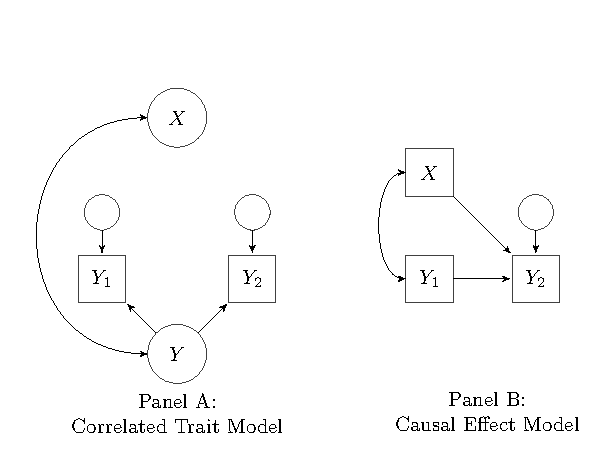
\includegraphics{images/dgm.pdf}
\caption{\label{fig:dgm}Two possible data-generating models that can produce indistinguishable correlation matrices. Panel A is a correlated-trait model with no causal effects; Panel B is a causal-effects model where X is correlated with Y1 but also has a causal effect on Y2.}
\end{figure}

Next, Sorjonen, Melin, et al. (2024) use an analysis that is equivalent to the CLPM to predict \emph{Y2} from \emph{X} and \emph{Y1}. They show that this analysis leads to a spurious path from \emph{X} to \emph{Y2} after controlling for \emph{Y1}, even though there is no causal effect in the data-generating model. In other words, the authors test and find support for the model in Panel B of Figure \ref{fig:dgm} (in which there is a true causal effect), despite the fact that the data were generated using the model shown in Panel A (where there is no causal effect).

Finally, they use their triangulation method to show that when the regression equation is reversed to predict \emph{Y1} from \emph{X} and \emph{Y2}, the coefficient for \emph{X} is positive. They then reason that if this coefficient is positive when the data were generated from a model with no causal effect, then the existence of this positive coefficient must signal a spurious effect. This conclusion, however, is incorrect. The existence of a positive coefficient when reversing the regression equation should only be interpreted as a signal of a spurious effect if the coefficient is positive \emph{if and only if} the estimated causal effect is spurious. Although we agree that the sign will be positive when the estimated causal effect is spurious, it will \emph{also} be positive in many cases where a \emph{true} causal effects exist. Thus, the triangulation method suffers from low specificity, as it provides false positives when evaluating CLPM findings.

The authors' own hypothetical example illustrates the problem with their approach. Panel B of Figure \ref{fig:dgm} is a diagram of a data-generating model that incorporates a true causal effect of a latent variable \emph{X} on \emph{Y2}. The problem with two-wave longitudinal studies is that the exact same correlation matrix can be consistent with these two very different underlying data-generating models, one that includes a causal effect and one that does not (Lucas, 2023). There is simply not enough information in the three correlations in this three-variable correlation matrix to distinguish between these two plausible models\footnote{Note that in their example, there is just one measure of \emph{X}. Adding an additional observation of \emph{X} at Time 2 does not help, though adding a third wave for both \emph{X} and \emph{Y} does (Lucas, 2023).}. And although it is true that the method proposed by Sorjonen, Melin, and colleagues will detect a spurious causal effect when the true data-generating model is that specified in Panel A; it will also necessarily detect a spurious effect when the true data-generating model is that specified in Panel B, where there is a true causal effect. Again, this is due to the fact that the correlation matrix underlying their regression tests will be the same in either case. Thus, although the proposed pattern of coefficients does emerge when estimated causal effects from the CLPM are spurious, this pattern will also emerge when true causal effects exist. Thus, the test is not diagnostic for spurious effects. In later sections, we conduct simulations to show what conditions affect these coefficients and explain these simulations by considering the links between coefficients in multiple regression and their underlying correlations.

\subsection{Detecting True Effects}\label{detecting-true-effects}

Recently, Sorjonen, Arshamian, et al. (2024) developed an additional line of argumentation to support the validity of their approach. Instead of showing that the procedure correctly identifies spurious results, in this paper, they used an experiment to demonstrate that the model can also correctly identify true causal effects. The experiment they conducted was straightforward: They began with cups filled with different amounts of water, and thus had had different weights. These initial weights serve as the initial measure of the outcome variable (\emph{Y1}). They then added different amounts of water to different cups, a manipulation (\emph{X1}) that has a causal effect on the final weight of the cups (\emph{Y2}). They showed that in this situation, their set of regression analyses correctly identified that the causal effect was not spurious. The effect of \emph{X1} on \emph{Y2} controlling for \emph{Y1} was positive, the effect of \emph{X1} on \emph{Y1} controlling for \emph{Y2} was negative, and the effect of \emph{X1} on the difference between \emph{Y2} and \emph{Y1} was positive. The authors argued that this demonstrates the validity of their approach.

We agree that in this situation, the pattern of coefficients that signals a true causal effect will emerge. However, this example highlights an important flaw in the approach. The CLPM estimates the effect of a predictor on an outcome, controlling for an earlier measure of this outcome. This procedure is used specifically to remove the effects of confounds that simultaneously affect the predictor and outcome. In other words, the CLPM is useful when the association between the predictor and outcome is confounded by some third variable; longitudinal data can help address some of these confounds (Rohrer \& Murayama, 2021). In the authors' example, there can be no confounds that need to be controlled. \emph{X1}, by design, is uncorrelated with the initial measure of \emph{Y}, so in this example, \emph{Y1} does not need to be controlled. Regressing \emph{Y2} on \emph{X1} recovers the true causal effect, even without controlling for the earlier measure of \emph{Y}.

This can be verified in the authors' own data (available here: \url{https://osf.io/dpvzr/}). We downloaded their data and tested a model predicting the final weight of the cups (i.e., \emph{Y2}) from the manipulation (amount added; i.e., \emph{X1}) and the resulting coefficient was 14.33. The coefficient from a model that controls for \emph{Y1}, initial weight (which is, of course, highly correlated with the outcome), was 14.40 (these estimates are not identical because there was measurement error and thus, the correlation between the two predictors was not precisely 0). In other words, this example demonstrates that the method for detecting spurious causal effects works \emph{in a situation where the CLPM would not be needed}. As with the hypothetical examples used in earlier papers, this example does not speak to whether the method can distinguish true from spurious effects.

\subsection{Simulating Different Data-Generating Models}\label{simulating-different-data-generating-models}

To clarify when the proposed test for spuriousness incorrectly detects true causal effects as spurious, we simulated data from a broad range of data-generating models. Specifically, we generated data that varied in: (a) how strongly the initial predictor and outcome were correlated, (b) how stable the outcome variable was, (c) the size of the cross-lagged effect, and (d) how much residual variance there was in the final measure of the outcome variable. These are not the only parameters we could simulate, but we believe that, together, they highlight some of the critical problems with the triangulation method.

We created a function to generate data according to the four parameters described above (all code for the simulation is available at our OSF site: \url{https://osf.io/u49q5/}). We generated data for four values of the initial correlation (0, .3, .6, and .9), five values of the stability coefficient (0, .25, .50, .75, and 1), five values of the cross-lagged effect (0, .25, .50, .75, and 1), and three values of the residual variance (.3, .6, and .9). For all parameters, we wanted to examine a broad range of values that ranged from no association to a strong association. For the initial correlation we did not include a value of 1 because it did not make sense to include a model where the predictor and initial outcome were perfectly correlated. Therefore, we included equally spaced values from 0 to .9. For the stability and cross-lagged effects we did want to include both 0 and 1 to capture associations ranging from no effect to an effect where a one unit change in the predictor leads to a one-unit change in the outcome. Therefore, we included five equally spaced values from 0 to 1. For the residual variance, the meaning of the specific values depends on the standard deviation of the simulated variables. The standard deviation for the predictor and initial measure of the outcome were set to be 1; the relative contribution of the residual variance depends on the size of the corresponding stability and cross-lagged paths. We created 20 datasets, each with a sample of 10,000 simulated participants, for each set of the 300 possible combinations of these four parameters. For simplicity sake, we only simulated variables that were positively correlated with one another (or uncorrelated). Because the triangulation procedure involves predictions of sign reversals, it is easier to keep track of these predictions if all associations have the same sign. The principles we identify, however, generalize to situations where the variables have negative correlations.

\begin{figure}
\centering
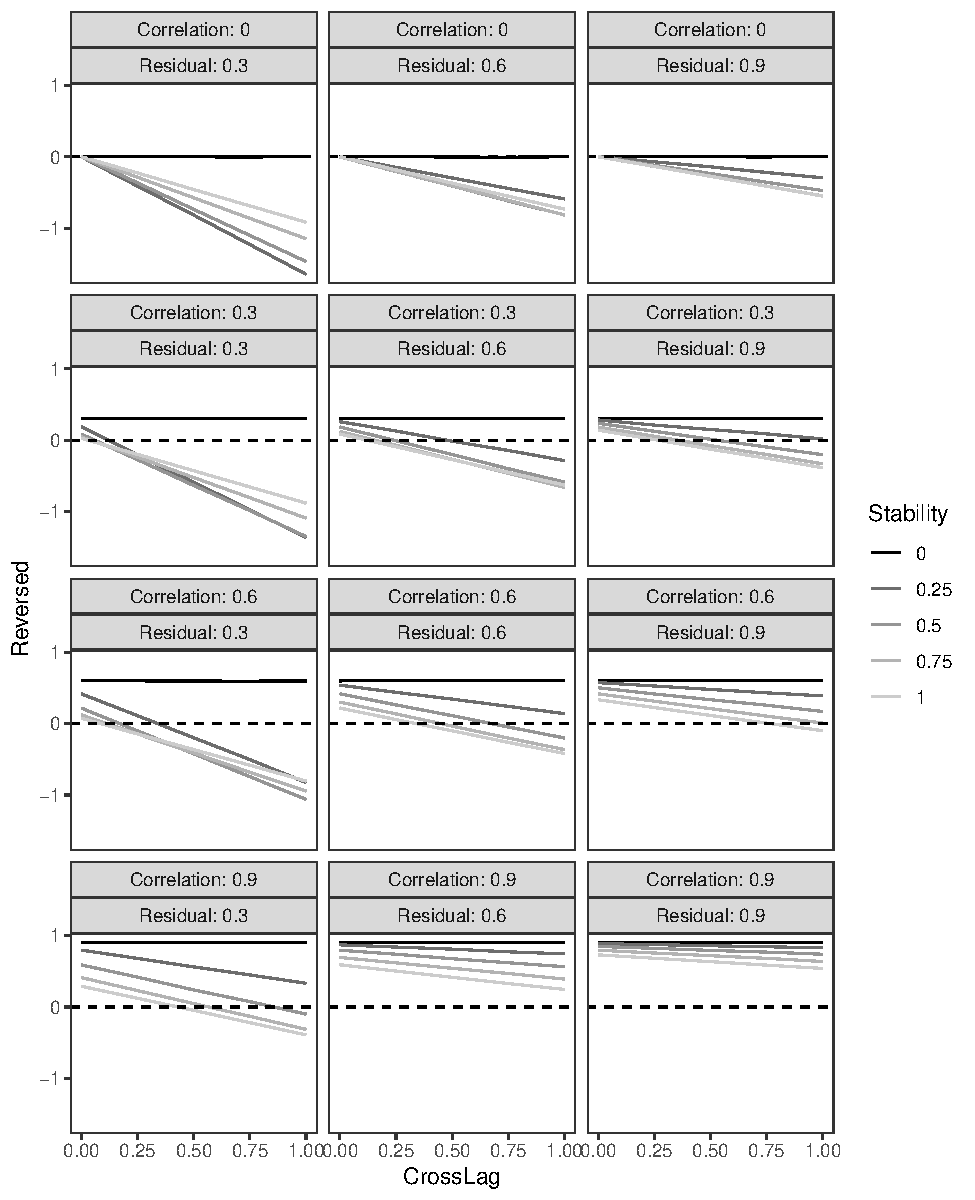
\includegraphics{triangulation_files/figure-latex/sim1-1.pdf}
\caption{\label{fig:sim1}Coefficients from the reversal test, predicting the initial measure Y1 from X1 and Y2. Correlation is the initial correlation between Y1 and X1. Residual is the residual variance of Y2.}
\end{figure}

We focus on the second and third tests from the triangulation method. The first step is not used to detect spuriousness (it is the typical estimate of the causal effect that one might suspect to be spurious) and it will be equivalent to the specified cross-lagged parameter value in our data-generating model because the regression equation that is being tested is identical to the data-generating model.

\subsubsection{Reversal Test}\label{reversal-test}

Figure \ref{fig:sim1} shows the simulations for the reversal test: the estimates for the reversed regression predicting \emph{Y1} from \emph{X1} and \emph{Y2}. Because all effects in this simulation were specified to be positive, this coefficient should be negative when true lagged effects exist according to the triangulation method. In other words, for all results in this figure (with the exception of the leftmost values in each panel, where the causal effect is 0), the reversal test specifies that the coefficients should be negative, due to the fact that there are true causal effects. The dashed line in the figure indicates a coefficient of zero, so anything above this line is a true causal effect that would be detected as spurious (i.e., as a false positive) when using the triangulation method.

Consistent with our argument above, this prediction for the reversal test only holds when the predictor and the initial measure of the outcome are uncorrelated. The correlations between \emph{X1} and \emph{Y1} are 0 for all simulations in Row 1 of the figure, and indeed, all coefficients are negative in this row. Remember, however, that when the predictor and outcome are uncorrelated, the CLPM would not need to be used as there are no confounds to control. The other rows show that as soon as a correlation between \emph{X1} and \emph{Y1} is introduced, positive coefficients are possible, even in the presence of true causal effects.

A slightly unrealistic (but not implausible) example highlights one reason why positive coefficients from the reversal test emerge when the \emph{X} and \emph{Y1} are correlated. Consider a case where \emph{X1} and \emph{Y1} are correlated .4, where there is a true effect of \emph{X1} on \emph{Y2} of .6, but there is no stability of \emph{Y} from \emph{Y1} to \emph{Y2} (independent of the stability due to the correlation between \emph{Y1} and \emph{X1} and the effect of \emph{X1} on \emph{Y}). We simulated data from this data-generating model (with \emph{X1} and \emph{Y1} having a mean of 0 and SD of 1 and \emph{Y2} having a residual variance of .5), which resulted in the correlation matrix in the top panel of Table \ref{tab:example}.

\begin{table}
\caption{\label{tab:example}Estimates from the Reversal test when the stability of Y is 0. The first panel shows the correlation matrix; the second panel shows the standard test from the CLPM; the third panel shows the results of the reversal test.}

\centering
\begin{tabular}[t]{lrrr}
\toprule
  & Y1 & X & Y2\\
\midrule
Y1 & 1.00 & 0.38 & 0.29\\
X & 0.38 & 1.00 & 0.76\\
Y2 & 0.29 & 0.76 & 1.00\\
\bottomrule
\end{tabular}
\centering
\begin{tabular}[t]{lrr}
\toprule
term & estimate & std.error\\
\midrule
(Intercept) & 0.0 & 0.00\\
X & 0.6 & 0.01\\
Y1 & 0.0 & 0.01\\
\bottomrule
\end{tabular}
\centering
\begin{tabular}[t]{lrr}
\toprule
term & estimate & std.error\\
\midrule
(Intercept) & 0.01 & 0.01\\
X & 0.39 & 0.01\\
Y2 & -0.01 & 0.02\\
\bottomrule
\end{tabular}
\end{table}

If you fit a regression model to these data predicting \emph{Y2} from \emph{Y1} and \emph{X1}, you recover the parameters from the data-generating model (the coefficient for \emph{X1} is 0.60 and for \emph{Y1} is 0.00). However, if you conduct the reversal test from the triangulation method, the coefficient for \emph{X1} predicting \emph{Y1}, controlling for \emph{Y2} is 0.39. In this model, we know there is actually a causal effect (because we specified it in the data-generating model), but the prediction of a negatively signed coefficient for a true effect is not confirmed. The reason is that if there is a correlation between \emph{X1} and \emph{Y1}, but \emph{Y2} is uncorrelated with \emph{Y1} (independent of \emph{X1}), the reversal regression reduces to an estimate of the zero-order correlation between \emph{X1} and \emph{Y1} (in this case, 0.38; the estimate is not exactly the same because of measurement error in \emph{Y2}). The solid black line in each panel of Figure \ref{fig:sim1} represents the models where stability was 0, and in these cases, the coefficient from the reversal test is always equal to the correlation between \emph{X1} and \emph{Y1}, regardless of the other parameters used to simulate the data.

Indeed, this example provides hints as to why the reversal test of spuriousness fail. Consider the equation for a regression coefficient, a discussion of which can help with the interpretation of the coefficient from the reversal test. The formula linking the underlying correlations (predicting \emph{Y1} from \emph{X1} controlling for \emph{Y2}) to the coefficient is as follows: \[\beta_{R} = \frac{r_{X1,Y1} - r_{Y1,Y2} \times r_{X1,Y2}} {1 - r_{X1,Y2}^{2}}\] In this equation, \(r_{X1,Y1}\) is the correlation between \emph{X1} and \emph{Y1}, \(r_{Y1,Y2}\) is the correlation between \emph{Y1} and \emph{Y2} (the stability of Y), and \(r_{X1,Y2}\) is the correlation between \emph{X1} and \emph{Y2} (or the correlation between the two predictors in the model for the reversal test).

The sign of this coefficient---a critical test in the triangulation method---will be determined by the numerator of this equation. In the case that Sorjonen, Arshamian, et al. (2024) highlight, the case of a true experiment, \(r_{X1,Y1}\) will be 0, which means that the coefficient will be negative (unless one other pair of variables is also uncorrelated, in which case, it will be 0). In the case we highlighted, where the stability of the \emph{Y} variables is 0, the second term in the numerator will reduce to zero, resulting in a coefficient that is equivalent to the correlation between \emph{X1} and \emph{Y1}. This equation shows that---holding the correlation between \emph{X1} and \emph{Y1} constant---anything that reduces the second term in the numerator will make the coefficient less negative/more positive. In other words, for (positively) correlated predictors in a standard CLPM, the coefficient for this reversal test will be more likely to be positive as (a) stability of the outcome measure decreases, (b) the true cross-lagged effect decreases, and (c) the amount of residual variance in the Time 2 outcome increases (which would reduce the correlation between the Time 2 outcome and either variable in the model). Each of these patterns can be seen in Figure \ref{fig:sim1}\footnote{Note that the patterns of increasing or decreasing coefficients are mostly consistent across panels of Figure \ref{fig:sim1}, but there are some exceptions when the correlations between \emph{X1} and \emph{Y1} are weak and when the residual variance in \emph{Y2} is low. This appears to be due to the scaling factor (the denominator) in the equation for regression coefficients.}.

One response to our critique of the triangulation method might be to highlight that although it is not \emph{necessarily} true that spurious effects will lead to negative coefficients, they might \emph{often} do so. Indeed, for many panels in Figure \ref{fig:sim1}, the majority of simulated coefficients were negative, especially as the true causal effect increased in size. However, this argument requires some knowledge about which of the parameter values we used in the simulation matches reality, and that is something that we believe is unknowable at this time. In fact, Orth et al. (2022) meta-analytically summarized effect sizes from cross-lagged panel studies, and the vast majority of these effects were below .12, which was the 75th percentile for effects. Focusing only on the simulated coefficients for true causal effects of this size, positive coefficients are common.

\subsubsection{Difference Test}\label{difference-test}

Figure \ref{fig:sim2} shows the results for the \emph{difference test} proposed by the proponents of the triangulation method, in which the difference between \emph{Y2} and \emph{Y1} is regressed on \emph{X1}. In this case, the prediction is that for true effects, this coefficient should be positive. The equation for the regression coefficient for the difference test is (Sorjonen, Melin, et al., 2024): \[\beta_{D} = \frac{r_{X1,Y2} - r_{X1,Y1}} {\sqrt{2(1 - r_{Y1,Y2})}}\] Again, the sign of this test is determined by the numerator of the equation, and it will be negative (signaling a spurious effect) when the correlation \(r_{X1,Y2}\) is smaller than the correlation \(r_{X1,Y1}\). This can happen in the presence of true causal effects if there is a substantial correlation between \emph{X1} and \emph{Y1}, low stability from \emph{Y1} to \emph{Y2}, and weak effects of \emph{X1} on \emph{Y2}. The simulations shown in Figure \ref{fig:sim2} highlight these patterns. The factors that lead to negative coefficients in the presence of true causal effects are: stronger correlations between \emph{X1} and \emph{Y1}, smaller true causal effects of \emph{X1}, and weaker stability of \emph{Y}. The effect of increasing residual variance in \emph{Y2} is less pronounced as compared to the effect for the reversal test. Again, these simulations (and the formula for the regression coefficient) show that the difference test is not diagnostic of spurious effects.

\begin{figure}
\centering
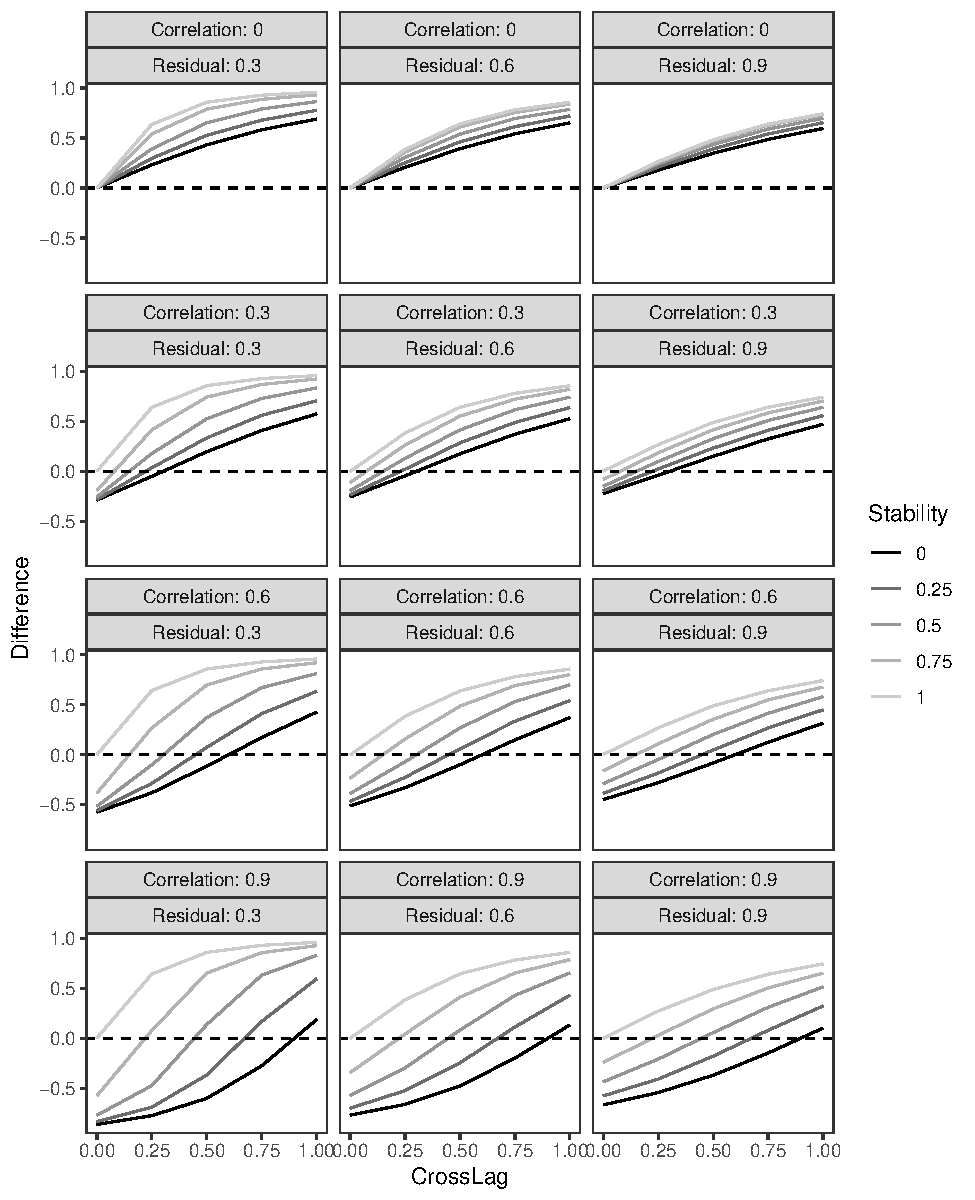
\includegraphics{triangulation_files/figure-latex/sim2-1.pdf}
\caption{\label{fig:sim2}Coefficients from the difference test, predicting the difference between \emph{Y2} and \emph{Y1} from \emph{X1}. Correlation is the initial correlation between \emph{X1} and \emph{Y1}; residual is the residual variance in \emph{Y2}.}
\end{figure}

\subsection{Discussion}\label{discussion}

Methodologists and researchers who use quantitative methods in applied settings will prefer to use methods that provide answers to theoretically interesting questions as efficiently as possible\footnote{To be clear, we are using the term ``efficient'' not in the statistical sense but in the common-language sense in which a task is accomplished more quickly and with fewer resources.}. The CLPM has been widely used precisely because it requires so little---just two variables assessed on two occasions---to do so much. The hope is that simply by controlling for prior measures of an outcome variable, most of the confounding effect off third variables can be controlled, resulting in unbiased estimates of causal effects. Unfortunately, the method is not up to this task; because of unmeasured heterogeneity and other statistical issues, estimated lagged effects can often be found, even when no true causal effect exists (Hamaker et al., 2015; Lucas, 2023).

Sorjonen, Melin, and their colleagues proposed a triangulation method that maintains the efficiency of the CLPM, while purportedly providing additional evidence about whether the estimates from this model are spurious or not. If valid, this approach would solve a critical problem in the field, as most other solutions to the statistical problems of the CLPM require additional waves of data (e.g., Hamaker et al., 2015), making them more data intensive, more expensive, and less efficient than the CLPM (at least with its minimal requirements). Unfortunately, the triangulation method cannot be used to diagnose spurious effects. The problem is that the same correlation matrix---in particular, one that is consistent with a spurious effect resulting from regression to the mean or the effects of unobserved heterogeneity---can also be consistent with a data-generating process that includes a true causal effect. Thus, conclusions about whether a specific effect is spurious should not be drawn from the triangulation method.

In this paper, we used simulations and the formulas for regression coefficients from multiple-regression analyses to show that predictions from the triangulation method are only guaranteed to hold in situations where the CLPM and related methods are not needed---when the initial measures of the two variables under investigation are not correlated. As soon as a correlation between these two variables is introduced, which is precisely when models like the CLPM and its more sophisticated alternatives are needed, the predictions from the proposed triangulation method will not hold. Specifically, when these variables are correlated, the predicted negative coefficient from the reversal test will become more positive as (a) the stability of the outcome gets weaker, (b) the true causal effect gets smaller, and (c) (in most cases) as more residual variance is included in the subsequent measure of the outcome. Importantly, the parameter values chosen for our simulations cover a range of arguably realistic values.

We want to be clear that our critique of the triangulation method should not be interpreted as a defense of the CLPM or studies that use it. Like the authors of the triangulation method, we believe that the use of the CLPM is likely to lead to evidence for causal effects when they do not exist, due to regression to the mean and unobserved heterogeneity. However, the triangulation method does not add information about the likelihood that an effect is spurious. The pattern of results that the authors claim provides evidence for spuriousness is equally consistent with data-generating models that include true causal effects as those for which no such effects exist.

In short, although the goals of the triangulation method are commendable, the method does not provide valid evidence about whether an effect from the CLPM is spurious or not. The advocates of this approach have published many papers reanalyzing data from publications that used the CLPM, typically concluding that those results were spurious. Because of widely known limitations of the CLPM, we do not wish to defend the conclusions from the original papers. However, the application of the triangulation method to them does not provide any new information, and claims about spuriousness are not justified.

\subsection{Author Contributions}\label{author-contributions}

Richard E. Lucas conceptualized the study and wrote the initial analysis code and the first draft of the paper.

Rebekka Weidmann and Mark Brandt contributed to the conceptualization and edited the text.

\subsection{Conflicts of Interest}\label{conflicts-of-interest}

The authors declare that there were no conflicts of interest with respect to the authorship or the publication of this article.

\subsection{Prior Versions}\label{prior-versions}

A preprint of this paper was posted on the PsyArXiv preprint server: \url{https://osf.io/u49q5/}.

\newpage

\section*{References}\label{references}
\addcontentsline{toc}{section}{References}

\phantomsection\label{refs}
\begin{CSLReferences}{1}{0}
\bibitem[\citeproctext]{ref-berry_practical_2017}
Berry, D., \& Willoughby, M. T. (2017). On the {Practical Interpretability} of {Cross-Lagged Panel~Models}: {Rethinking} a {Developmental Workhorse}. \emph{Child Development}, \emph{88}(4), 1186--1206. \url{https://doi.org/gbf8jt}

\bibitem[\citeproctext]{ref-dishop_tutorial_2021}
Dishop, C. R., \& DeShon, R. P. (2021). A tutorial on {Bollen} and {Brand}'s approach to modeling dynamics while attending to dynamic panel bias. \emph{Psychological Methods}. \url{https://doi.org/10.1037/met0000333}

\bibitem[\citeproctext]{ref-duncan_linear_1969}
Duncan, O. D. (1969). Some linear models for two-wave, two-variable panel analysis. \emph{Psychological Bulletin}, \emph{72}(3), 177--182. \url{https://doi.org/10.1037/h0027876}

\bibitem[\citeproctext]{ref-finkel_causal_1995}
Finkel, S. E. (1995). \emph{Causal {Analysis} with {Panel Data}}. Thousand Oaks, CA: Sage Publications, Inc.

\bibitem[\citeproctext]{ref-hamaker_critique_2015}
Hamaker, E. L., Kuiper, R. M., \& Grasman, R. P. P. P. (2015). A critique of the cross-lagged panel model. \emph{Psychological Methods}, \emph{20}(1), 102--116. \url{https://doi.org/f67cvh}

\bibitem[\citeproctext]{ref-heise_causal_1970}
Heise, D. R. (1970). Causal {Inference} from {Panel Data}. \emph{Sociological Methodology}, \emph{2}, 3--27. \url{https://doi.org/10.2307/270780}

\bibitem[\citeproctext]{ref-kim_gain_2021}
Kim, Y., \& Steiner, P. M. (2021). Gain {Scores Revisited}: {A Graphical Models Perspective}. \emph{Sociological Methods \& Research}, \emph{50}(3), 1353--1375. \url{https://doi.org/10.1177/0049124119826155}

\bibitem[\citeproctext]{ref-krauss_work_2022}
Krauss, S., \& Orth, U. (2022). Work {Experiences} and {Self-Esteem Development}: {A Meta-Analysis} of {Longitudinal Studies}. \emph{European Journal of Personality}, \emph{36}(6), 849--869. \url{https://doi.org/10.1177/08902070211027142}

\bibitem[\citeproctext]{ref-lucas_why_2023}
Lucas, R. E. (2023). Why the {Cross-Lagged Panel Model Is Almost Never} the {Right Choice}. \emph{Advances in Methods and Practices in Psychological Science}, \emph{6}(1). \url{https://doi.org/10.1177/25152459231158378}

\bibitem[\citeproctext]{ref-ludtke_comparison_2022}
Lüdtke, O., \& Robitzsch, A. (2022). \emph{A comparison of different approaches for estimating cross-lagged effects from a causal inference perspective}. PsyArXiv. \url{https://doi.org/10.31234/osf.io/gcvb4}

\bibitem[\citeproctext]{ref-orth_effect_2022}
Orth, U., Meier, L., L., Buhler, J. L., Dapp, L. C., Krauss, S., Messerli, D., \& Robins, R. W. (2022). Effect {Size Guidelines} for {Cross-Lagged Effects}. \emph{Psychological Methods}.

\bibitem[\citeproctext]{ref-ployhart_two_2014}
Ployhart, R. E., \& MacKenzie, W. I. (2014). Two {Waves} of {Measurement Do Not} a {Longitudinal Study Make}. In C. E. Lance \& R. J. Vandenberg (Eds.), \emph{More {Statistical} and {Methodological Myths} and {Urban Legends}} (pp. 85--99). Routledge.

\bibitem[\citeproctext]{ref-rogosa_myths_1995}
Rogosa, D. R. (1995). Myths and methods: "{Myths} about longitudinal research" plus supplemental questions. In J. M. Gottman (Ed.), \emph{The {Analysis} of {Change}} (pp. 3--66). Mahwah, NJ: Lawrence Erlbaum Associates.

\bibitem[\citeproctext]{ref-rohrer_these_2021}
Rohrer, J. M., \& Murayama, K. (2021). These are not the effects you are looking for: {Causality} and the within-/between-person distinction in longitudinal data analysis. \emph{Advances in Methods and Practices in Psychological Science}, \emph{6}(1). \url{https://doi.org/10.1177/25152459221140842}

\bibitem[\citeproctext]{ref-sorjonen_aqua_2024}
Sorjonen, K., Arshamian, A., Lager, E., Nilsonne, G., \& Melin, B. (2024). \emph{In aqua veritas: {Triangulation} of cross-lagged effects for improved causal inference}. OSF. \url{https://doi.org/10.31234/osf.io/ztwy6}

\bibitem[\citeproctext]{ref-sorjonen_prospective_2022}
Sorjonen, K., Ingre, M., Melin, B., \& Nilsonne, G. (2022a). \emph{Prospective associations between self-esteem and quality of social relations may be spurious: {Reanalysis} of a meta-analysis of longitudinal studies}. \url{https://doi.org/10.31234/osf.io/kusft}

\bibitem[\citeproctext]{ref-sorjonen_questioning_2022}
Sorjonen, K., Ingre, M., Melin, B., \& Nilsonne, G. (2022b). \emph{Questioning the reciprocal effects model of academic self-concept and achievement: {A} reanalysis of a meta-analysis of longitudinal studies and a simulation}. \url{https://doi.org/10.31234/osf.io/qd4bj}

\bibitem[\citeproctext]{ref-sorjonen_questioning_2024}
Sorjonen, K., Ingre, M., Melin, B., \& Nilsonne, G. (2024). \emph{Questioning the reciprocal effects model of academic self-concept and achievement: {A} reanalysis of a meta-analysis of longitudinal studies and a simulation}. \url{https://doi.org/10.31234/osf.io/qd4bj}

\bibitem[\citeproctext]{ref-sorjonen_prospective_2023}
Sorjonen, K., \& Melin, B. (2023a). Prospective associations between social support and posttraumatic stress disorder may be spurious: {A} re-meta-analysis of longitudinal studies and a simulation. \emph{Journal of Affective Disorders}, \emph{340}, 174--180. \url{https://doi.org/10.1016/j.jad.2023.08.014}

\bibitem[\citeproctext]{ref-sorjonen_spurious_2023-2}
Sorjonen, K., \& Melin, B. (2023b). \emph{Spurious prospective effect of perfectionism on depression: {Reanalysis} of a meta-analytic cross-lagged panel analysis}. \url{https://doi.org/10.31234/osf.io/rfs3u}

\bibitem[\citeproctext]{ref-sorjonen_spurious_2023-1}
Sorjonen, K., \& Melin, B. (2023c). \emph{Spurious prospective effect of self-efficacy on academic performance: {Reanalysis} of a meta-analytic cross-lagged panel analysis}. \url{https://doi.org/10.31234/osf.io/qgcu5}

\bibitem[\citeproctext]{ref-sorjonen_prospective_2024}
Sorjonen, K., \& Melin, B. (2024a). Prospective effects of mindfulness on anxiety and depressive symptoms may be spurious: {Simulated} reanalysis of a meta-analytic cross-lagged panel analysis. \emph{PLOS ONE}, \emph{19}(5), e0302141. \url{https://doi.org/10.1371/journal.pone.0302141}

\bibitem[\citeproctext]{ref-sorjonen_spurious_2024-2}
Sorjonen, K., \& Melin, B. (2024b). Spurious prospective effects between general and domain-specific self-esteem: {A} reanalysis of a meta-analysis of longitudinal studies. \emph{PLOS ONE}, \emph{19}(2), e0298158. \url{https://doi.org/10.1371/journal.pone.0298158}

\bibitem[\citeproctext]{ref-sorjonen_spurious_2024}
Sorjonen, K., Melin, M., \& Melin, B. (2024). Spurious prospective effects between work experiences and self-esteem: {A} reanalysis of a meta-analysis of longitudinal studies. \emph{European Journal of Personality}, \emph{38}(3), 534--543. \url{https://doi.org/10.1177/08902070231197876}

\bibitem[\citeproctext]{ref-sorjonen_questioning_2022-1}
Sorjonen, K., Nilsonne, G., Ingre, M., \& Melin, B. (2022). Questioning the vulnerability model: {Prospective} associations between low self-esteem and subsequent depression ratings may be spurious. \emph{Journal of Affective Disorders}, \emph{315}, 259--266. \url{https://doi.org/10.1016/j.jad.2022.08.003}

\bibitem[\citeproctext]{ref-sorjonen_distorted_2023}
Sorjonen, K., Nilsonne, G., \& Melin, B. (2023a). Distorted meta-analytic findings on peer influence: {A} reanalysis. \emph{Heliyon}, \emph{9}(11), e21458. \url{https://doi.org/10.1016/j.heliyon.2023.e21458}

\bibitem[\citeproctext]{ref-sorjonen_spurious_2023}
Sorjonen, K., Nilsonne, G., \& Melin, B. (2023b). \emph{Spurious peer influence: {Reanalysis} of a meta-analysis of longitudinal studies}. \url{https://doi.org/10.31234/osf.io/szkt8}

\bibitem[\citeproctext]{ref-zyphur_data_2020}
Zyphur, M. J., Allison, P. D., Tay, L., Voelkle, M. C., Preacher, K. J., Zhang, Z., \ldots{} Diener, E. (2020). From {Data} to {Causes I}: {Building A General Cross-Lagged Panel Model} ({GCLM}). \emph{Organizational Research Methods}, \emph{23}(4), 651--687. \url{https://doi.org/gf8rt5}

\end{CSLReferences}


\end{document}
